% additional usepackage{beamerthemeshadow} is used
\documentclass{beamer}
\usepackage{beamerthemeshadow}
%\usepackage[style=apa,backend=biber]{biblatex}
%\addbibresource{slide.bib}
%\usepackage{hyperref}
%\usepackage{apacite}
\usepackage{natbib}
\def\newblock{}
\let\Tiny=\tiny

\begin{document}
%\let\@internalcite\citep
%\def\citep{\def\citepname##1{##1}\@internalcite}
%\def\@biblabel#1{\def\citepname##1{##1}[#1]\hfill}}

\title{Chinese Named Entity Recognition using Conditional Random Fields}
\author{Xilun Chen\inst{1}\inst{2}
%\footnote{\scriptsize On his visiting at Natural Language Computing Group, Microsoft Research Asia}
\and Yuanfei Zhu\inst{1} \and Zeyu Wang\inst{1}}
\institute{\inst{1}Shanghai Jiao Tong University
\and \inst{2}On his visiting at Microsoft Research Asia
}
\date{\today}

\frame{\titlepage}

\frame{\frametitle{Table of contents}\tableofcontents}

\section{Introduction}
\frame{\sectionpage}

\subsection{Named Entity Recognition}
\frame{\subsectionpage}

\frame{\frametitle{Named Entity Recognition}
\begin{itemize}
	\item NER is a task aimed at extracting named entities from raw text and classifying into their corresponding categories, such as persons, locations, organizations, etc. \pause
	\item In this task, we are required to identify three entity categories: PER, LOC, ORG given a Chinese text.
\end{itemize}
}

\frame{\frametitle{NER as a Sequence Labeling Task}
Sequence Labeling has been the state-of-the-art approach to a number of NLP tasks:
\begin{itemize}
	\item Word Segmentation\citep{tseng2005conditional}.
	\item	POS Tagging\citep{toutanova2000enriching}.
	\item	Chunking(Shallow Parsing)\citep{sha2003shallow}.
	\item Named Entity Recognition\citep{mccallum2003early}.
\end{itemize}
}

\subsection{Sequence Labeling}
\frame{\subsectionpage}

\frame{\frametitle{Sequence Labeling}
\tiny
\begin{block}{Hidden Markov Model (HMM)}
	\begin{itemize}
		\item Generative Model
		\item Cannot incorporate long distance features
	\end{itemize}
\end{block}
\begin{block}{Maximum Entropy Markov Model (MEMM)}
	\begin{itemize}
		\item Discriminative Model
		\item Can incorporate long distance features
		\item Optimize conditional probability
	\end{itemize}
\end{block}
\begin{block}{Conditional Random Field (CRF) --- \textit{Our Choice}}
	\begin{itemize}
		\item Discriminative Model
		\item Can incorporate long distance features
		\item Optimize joint probability (Has looser assumption of independency)
		\item High cost, long training time
	\end{itemize}
\end{block}
}

\section{Proposed Approach}

\frame{\sectionpage}

\subsection{Preprocessing}
\frame{\subsectionpage}

\frame{\frametitle{Tagging Scheme}
\begin{itemize}
	\item We need to convert the labels to fit the sequence labeling task.
		\pause
	\item We adopt the classic IOB tagging method with totally 7 tags: B-PER, I-PER, B-LOC, I-LOC, B-ORG, I-ORG and Others
		\pause
	\item Gain produced by more complex tagging methodologies like IOBES remains elusive.\citep{collobert2011natural}
\end{itemize}
}

\frame{\frametitle{Word Segmentation \& POS Tagging}
\small
\begin{block}{Word Segmentation}
	We adopt a word-based approach rather than character-based one under the rationale:
	\begin{itemize}
		\item In Chinese, words can better encode semantics atomics than characters.
		\item By word segmentation, additional useful features such as POS tags can be introduced.
	\end{itemize}
\end{block}

\begin{block}{POS Tagging}
	\begin{itemize}
		\item Named Entities are more likely to have particular POS tags (e.g. Proper Nouns).
		\item POS Tagging can ameliorate the problem of data sparsity.
	\end{itemize}
\end{block}
}

\subsection{Features}

\frame{\subsectionpage}

\frame{\frametitle{Lexical Features}
\begin{itemize}
	\item Lexical features are the most basic features that everyone would exploit.
		\pause
	\item But extravagant utilization of lexical features would result in severe sparsity problem.
		\pause
	\item Hence we incorporate some but limited lexical features of unigram, bigram and trigram features.
		\pause
	\item We also set a relatively large cutoff value to avoid the bias induced by lexical features of extremely low frequency.
\end{itemize}
}

\frame{\frametitle{POS Tags}
As we said before, POS tags can benefit the NER task.
\begin{itemize}
	\item Named Entities are very likely to possess a specific subset of POS tags (NR, for example).
		\pause
	\item POS tags does not suffer from the data sparsity as the lexical features.
\end{itemize}
}

\begin{frame}{Prefixes \& Suffixes}
	In Chinese, much helpful knowledge can be revealed by examining the prefix and suffix of a word.
	\pause
	\begin{itemize}
		\item e.g. Patterns like {\fontfamily{song} Zhang XX, Li XX suggests a high probability of persons.}
			\pause
		\item e.g. Patterns like XX Shi, XX Xian suggests a high probability of locations.
			\pause
		\item e.g. Patterns like XX Ju, XX Chu suggests a high probability of organizations.
	\end{itemize}
\end{frame}

\begin{frame}{Gazetteers}
	\citep{ratinov2009design} argued that numerous works have reported that gazetteers would substantially help the performance of a NER system.\citep{cohen2004exploiting,kazama2007exploiting,florian2003named}
	\pause
	\vspace{0.5cm}

	We collected a dozen of gazetteers from various sources (Experiments are still on-going, not final choice)
	\begin{itemize}
		\item A list of 300 most common Chinese Surnames
		\item Classified gazetteers from \textit{Sogou Cell Lexicon}.
	\end{itemize}
\end{frame}

\begin{frame}{Word Clustering}
	\begin{itemize}
		\item Word clustering is another approach that deals with the sparsity.
			\pause
		\item	Socher and Chris Manning from Stanford pointed out in their tutorial at ACL 2012\citep{socher2012deep} that Word Clustering can improve the accuracy of NER, as shown in Figure \ref{fig:cluster}.
	\end{itemize}
	\begin{figure}[h]
		\centering
		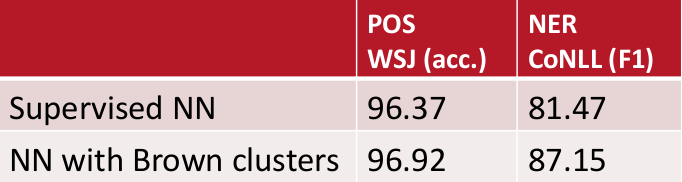
\includegraphics[height=0.25\textheight]{./figures/socher-clustering.png}
		\label{fig:cluster}
	\end{figure}
\end{frame}

\begin{frame}{Word Clustering (Cont.)}
	\begin{itemize}
		\item 
			We consider the classic Brown Clustering \citep{brown1992class}, with open source implementation by Percy Liang \citep{liang2005semi}.
			\pause
		\item We are also trying the \textbf{mkcls} clustering by Franz Josef Och \citep{och1999efficient}.
			\pause
		\item Another promising candidate is a Word Embedding trained by Deep Neural Networks \citep{turian2010word,collobert2011natural}, but we don't have enough time to train and test them.
	\end{itemize}
	\pause
	Experiments on Word Clustering are still on-going, and so far yield no promising results. (mkcls doesn't work well, and Brown takes too long time to train)
\end{frame}

\section{Experiments}
\subsection{Experiment Settings}
\frame{\sectionpage}

\begin{frame}{Experiment Settings}
	\begin{itemize}
		\item We use Stanford Segmenter\citep{tseng2005conditional} for word segmentation
			\pause
		\item We use Stanford POS Tagger\citep{toutanova2000enriching} for POS tagging.
			\pause
		\item We use CRF++ as implementation of CRF.
			\pause
		\item Data Selection:
			\begin{description}
				\item[Training Set] First 950/1000 documents in the training data.
				\item[Dev Set] Last 50/1000 documents in the training data.
			\end{description}
	\end{itemize}
\end{frame}

\begin{frame}{Sample Training Data}
	\begin{figure}[h]
		\centering
		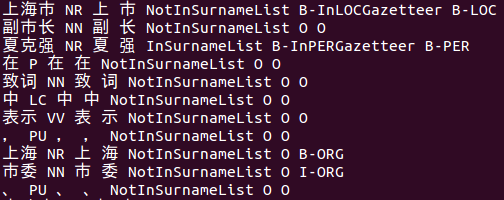
\includegraphics[width=0.8\textwidth]{./figures/traindata.png}
		\caption{Sample Training Data}
		\label{fig:traindata}
	\end{figure}
\end{frame}

\subsection{Results}
\frame{\frametitle{Results}
Table below shows the \textbf{Overall} F1 score on Dev Set.
%Term-level means a term would be counted as correct only if its boundary is precisely extracted.
\begin{tabular}{|c|c|c|}
	\hline
	\textbf{Setting} & \textbf{F1(Term-level)} & \textbf{F1(Character-level)} \\
	\hline
	Lexical & 66.91 & 67.51  \\
	\hline
	+POS & 79.02 & 81.95 \\
	\hline
	+Pre/Suffix & 85.99 & 88.89 \\
	\hline
	+Surname List & 87.61 & 89.40 \\
	\hline
	+Gazetteer & \textbf{88.84} & \textbf{90.31}\\
	\hline
\end{tabular}}

\frame{\frametitle{Results on PERSON}
Table below shows the F1 score of \textbf{PERSON} recognition.
%Term-level means a term would be counted as correct only if its boundary is precisely extracted.
\begin{tabular}{|c|c|c|}
	\hline
	\textbf{Setting} & \textbf{F1(Term-level)} & \textbf{F1(Character-level)} \\
	\hline
	Lexical & 42.51 & 41.94 \\
	\hline
	+POS & 71.30 & 79.52 \\
	\hline
	+Pre/Suffix & 79.95 & 86.44 \\
	\hline
	+Surname List & 85.01 & 88.06 \\
	\hline
	+Gazetteer & 86.46 & 89.26 \\
	\hline
\end{tabular}}

\frame{\frametitle{Results on LOCATION}
Table below shows the F1 score of \textbf{LOCATION} recognition.
%Term-level means a term would be counted as correct only if its boundary is precisely extracted.
\begin{tabular}{|c|c|c|}
	\hline
	\textbf{Setting} & \textbf{F1(Term-level)} & \textbf{F1(Character-level)} \\
	\hline
	Lexical & 79.32 & 76.79 \\
	\hline
	+POS & 84.52 & 83.61 \\
	\hline
	+Pre/Suffix & 89.59 & 89.74 \\
	\hline
	+Surname List & 90.21 & 90.62 \\
	\hline
	+Gazetteer & 91.46 & 91.85 \\
	\hline
\end{tabular}}

\frame{\frametitle{Results on ORGANIZATION}
Table below shows the F1 score of \textbf{ORGANIZATION} recognition.
%Term-level means a term would be counted as correct only if its boundary is precisely extracted.
\begin{tabular}{|c|c|c|}
	\hline
	\textbf{Setting} & \textbf{F1(Term-level)} & \textbf{F1(Character-level)} \\
	\hline
	Lexical & 65.90 & 73.19 \\
	\hline
	+POS & 78.74 & 82.28 \\
	\hline
	+Pre/Suffix & 86.85 & 89.94 \\
	\hline
	+Surname List & 85.66 & 89.22 \\
	\hline
	+Gazetteer & 86.51 & 89.59 \\
	\hline
\end{tabular}}

\subsection{Analysis}
\frame{\frametitle{Analysis \& Insights}
\begin{enumerate}
	\item LOCATION is a relatively easier task under our word-based system
		\pause
	\item PERSON has a lower accuracy.
		\pause
		\begin{itemize}
			\item A character based system may be more suitable for Chinese person name recognition. \pause
			\item Pre/Suffix and surname list incurred significant improvement in PERSON task. \pause
		\end{itemize}
	\item ORGANIZATION has a much better char-level F1 than term-level F1.
		\pause
		\begin{itemize}
			\item It is difficult to precisely judge the boundary of a ORG.
%				\pause
%				\begin{figure}[h]
%					\centering
%					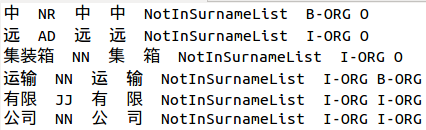
\includegraphics[height=0.2\textheight]{./figures/org.png}
%					\label{fig:discrepancyORG}
%				\end{figure}
		\end{itemize}
		\pause
	\item Gazetteers can bring noticeable improvement on every task despite its mediocre quality.
\end{enumerate}
}

\begin{frame}{The End}
	Thank you!
\end{frame}

{
\tiny
\bibliographystyle{apalike}
\bibliography{slide}
}

\end{document}
